\chapter{Astrolabium}

In dit hoofdstuk ga je aan de slag met het \textit{astrolabium}, een van de oudste navigatie-instrumenten. Je gebruikt het astrolabium zoals in figuur \ref{astrolabe-face}.

\begin{figure}
 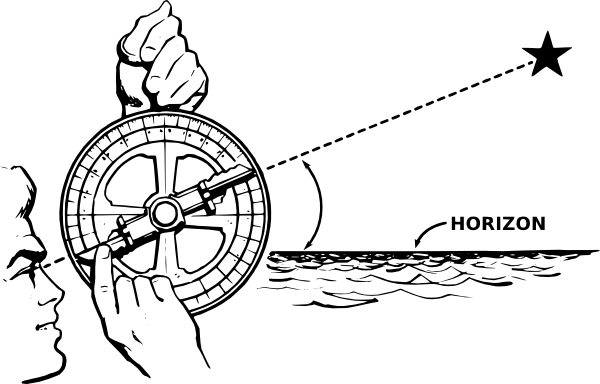
\includegraphics[width=0.7\textwidth]{astrolabe-hi.png}
 \label{astrolabe-face}
\end{figure}

Je bouwt eerst je eigen astrolabium, daarvoor krijg je een werkblad met de onderdelen van het astrolabium uitgedeeld. Allereerst kijken we naar de achterkant van het astrolabium (figuur \ref{astrolabe-back}).

\begin{figure}
 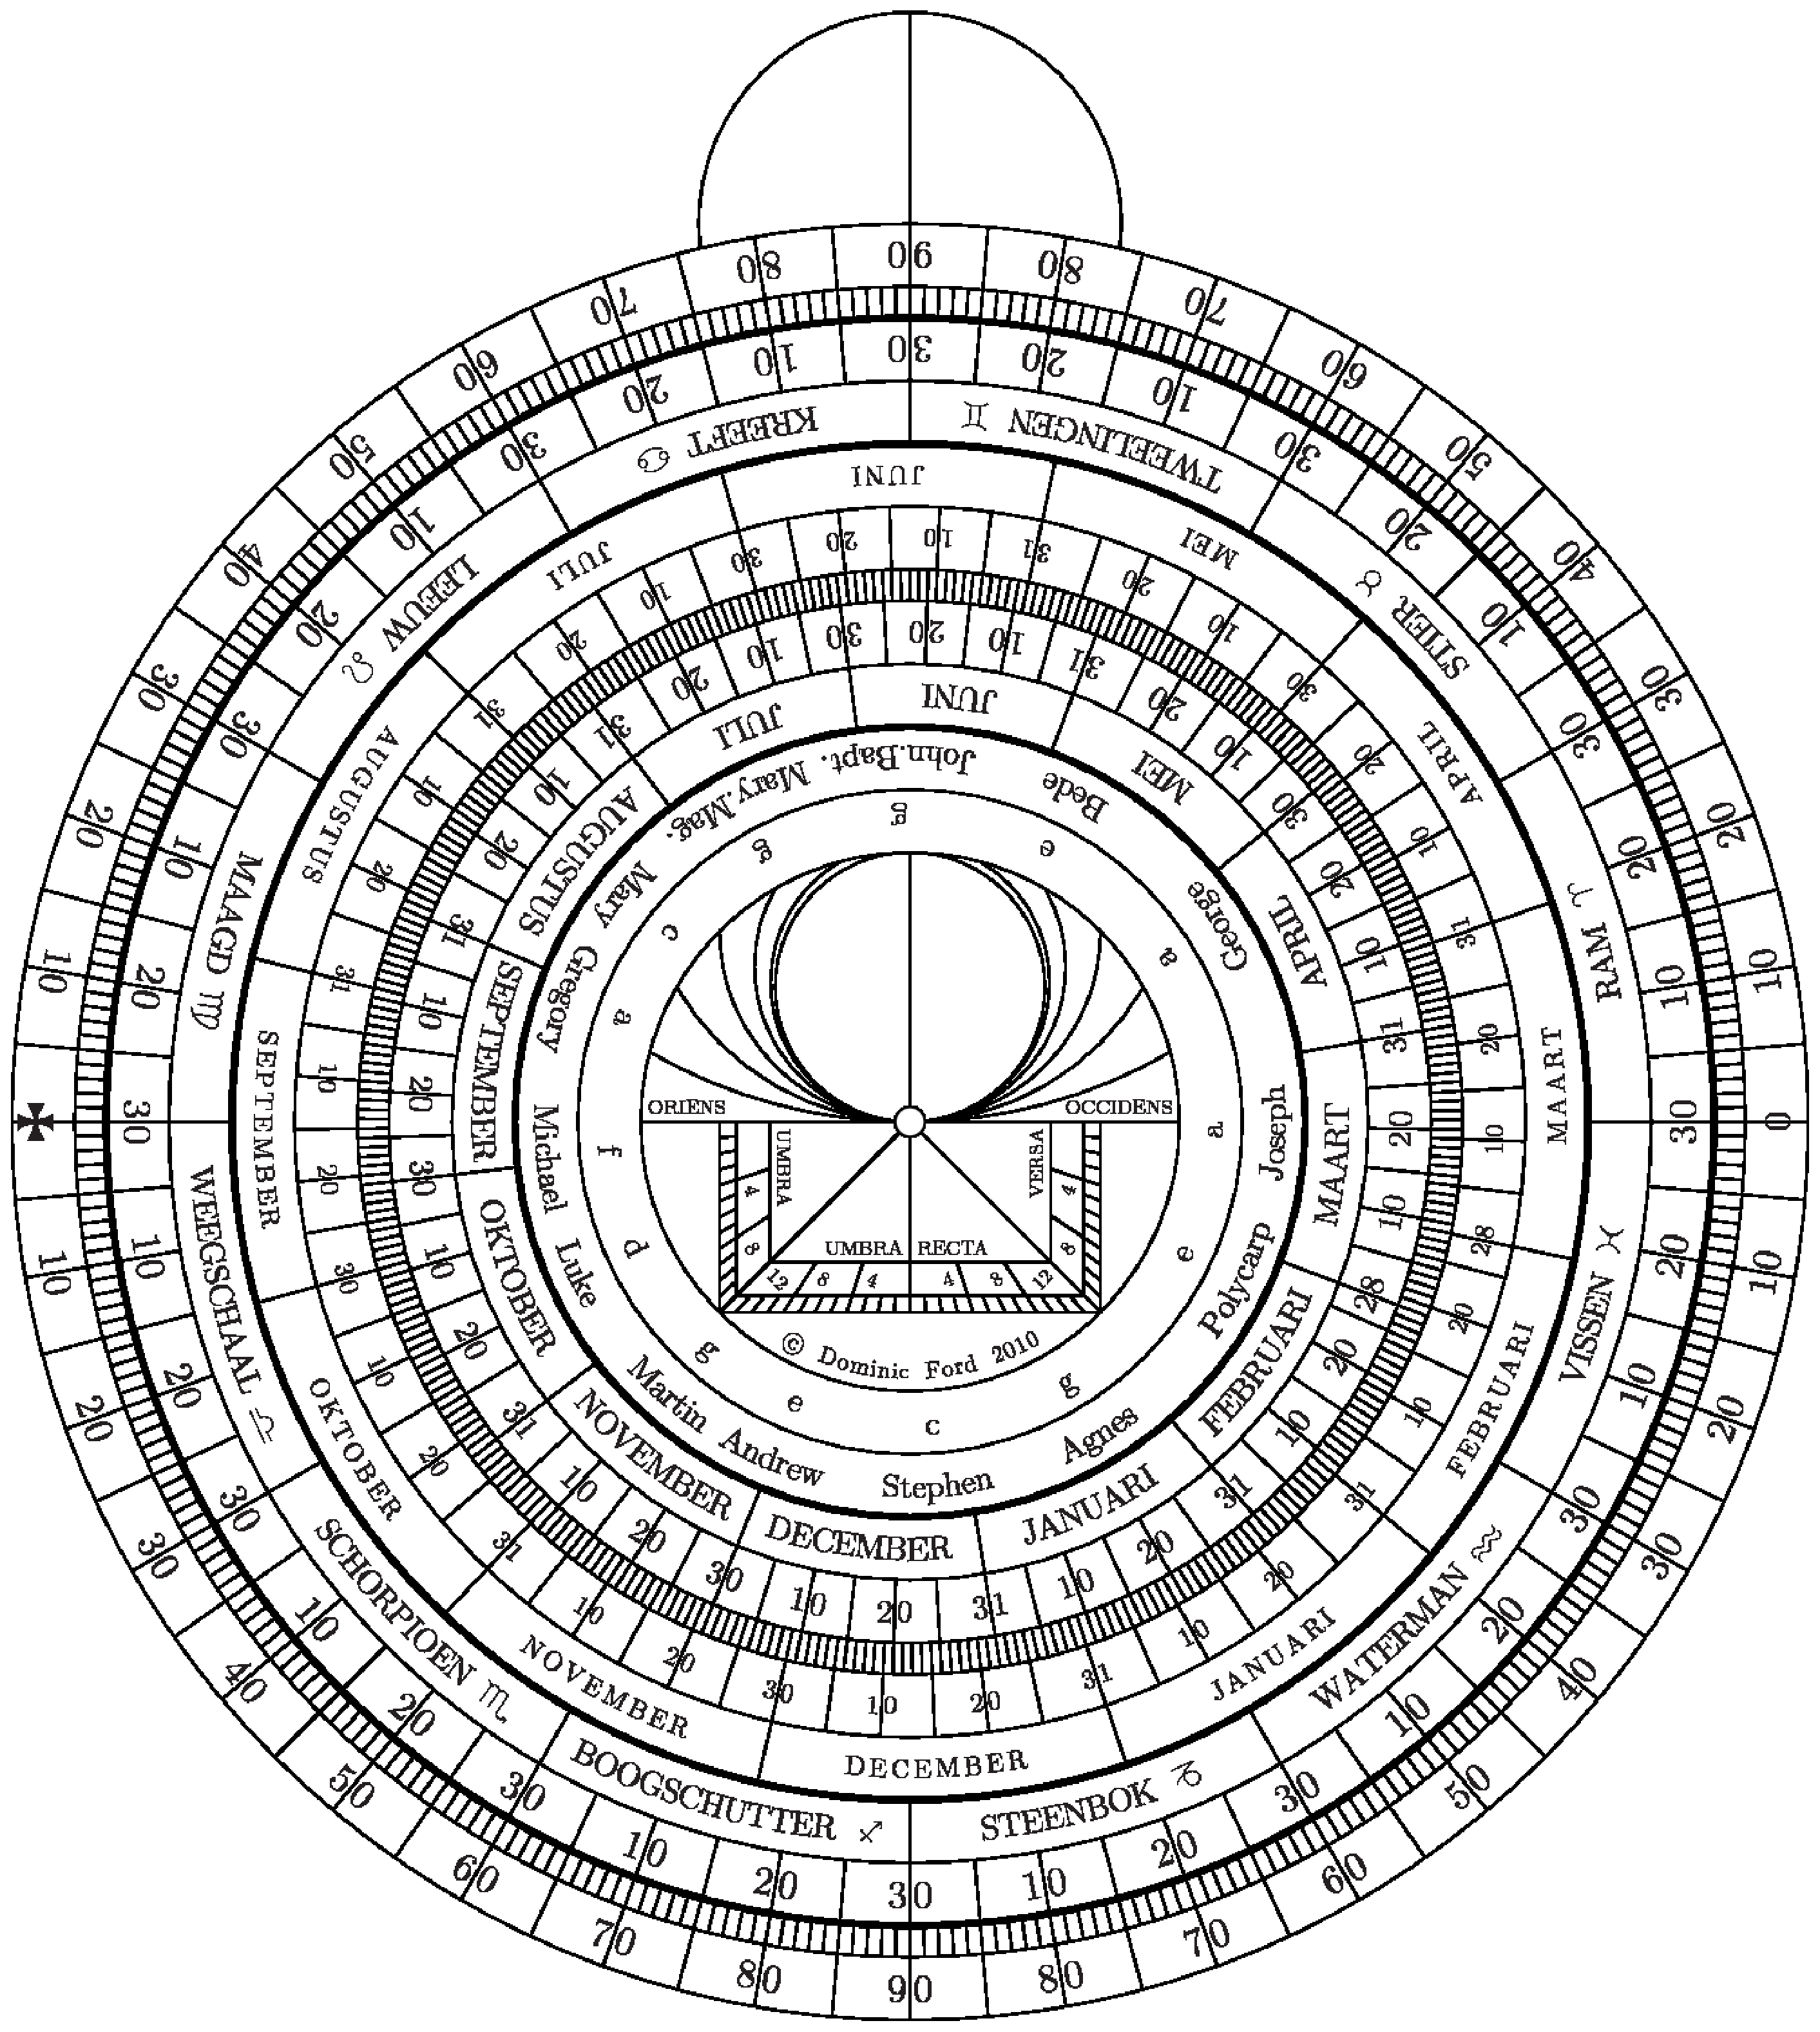
\includegraphics[width=0.7\textwidth]{astrolabiumNL/mother_back}
 \label{astrolabe-back}
 \caption{De achterkant van het astrolabium}
\end{figure}

De ringen, van buiten naar binnen, geven het volgende weer:
\begin{itemize}
 \item Schaal om de hoogte van een ster te bepalen.
 \item Dagen van de sterrenbeelden.
 \item Namen van de sterrenbeelden (de tekens van de dierenriem).
 \item Kalender passend bij het jaar 1394 (deze loopt negen dagen voor op de kalender voor onze tijd).
 \item Kalender passend bij onze eigen tijd.
 \item In de volgende twee ringen worden traditioneel de naamdagen van katholieke of anglicaanse heiligen weergegeven. Deze zijn weggelaten in ons astrolabium.
 \item De binnenste ring (schaduwschaal) zullen we niet gebruiken.
\end{itemize}

De alidade (figuur \ref{alidade}) draait over de achterkant van het astrolabium. \textcolor{red}{Naast de alidade op je werkblad wordt ook de \textit{rule} afgebeeld. Deze zullen we niet gebruiken.}

\begin{figure}
 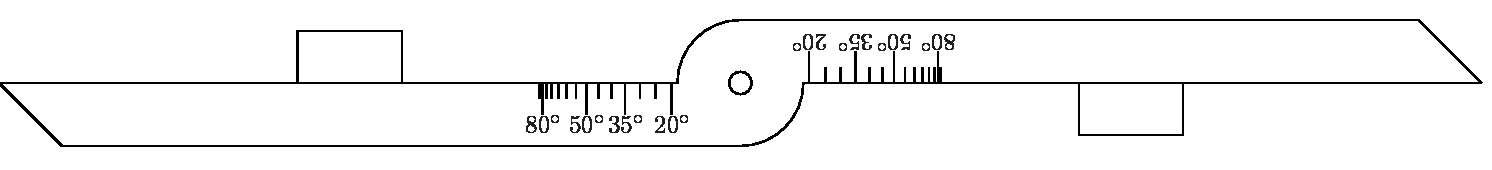
\includegraphics[width=0.7\textwidth]{astrolabiumNL/alidade}
 \label{alidade}
 \caption{De alidade}
\end{figure}

De voorkant van het astrolabium heeft het alfabet en een gradenboog rondom de \textit{plaat}. De plaat is gemaakt voor 52$^\circ$ Noorderbreedte, de breedtegraad van Nederland. Voor een andere breedtegraad heb je een andere plaat nodig. Het alfabet geeft de tijd aan, het kruis \kreuz is middernacht, de A is \'e\'en uur, de M is 12 uur 's middags, enzovoort.

Het laatste onderdeel, gemaakt van doorzichtig plastic, maar in vroeger tijden vaak een gouden of koperen plaat met veel uitsparingen, is de \textit{spin}. Op de spin staan een sterrenkaart en uren afgebeeld. 

De voorkant en de achterkant zijn niet helemaal cirkelvormig: aan de bovenkant zit nog een ring waaraan je het astrolabium kan vasthouden.

\begin{opgave}[\schaar]
 Knip nu alle onderdelen van het astrolabium uit. Lijm de voorkant en de achterkant op elkaar zodat de ring van beide onderdelen op elkaar zit, en je alle tekst kan lezen. Met een splitpen bevestig je de alidade op de achterkant en de spin op de voorkant van het astrolabium.
\end{opgave}
